\documentclass{standalone}

\usepackage{tikz}
\usetikzlibrary{arrows.meta, positioning, calc, backgrounds, fit, shapes}

% mcs --- memory consistency system. #1: name (an id number) for the node (also used in node text); #2: position
\newcommand{\mcs}[2]{\node (#1) [rectangle split,  rectangle split parts = 3, 
  rectangle split part fill = {white, white, white}, draw, text width = 2.5cm, align = center] at (#2) 
  {Processor $r_{#1}$: \nodepart{two} local memory \nodepart{three} DSM algorithm};}

\begin{document}

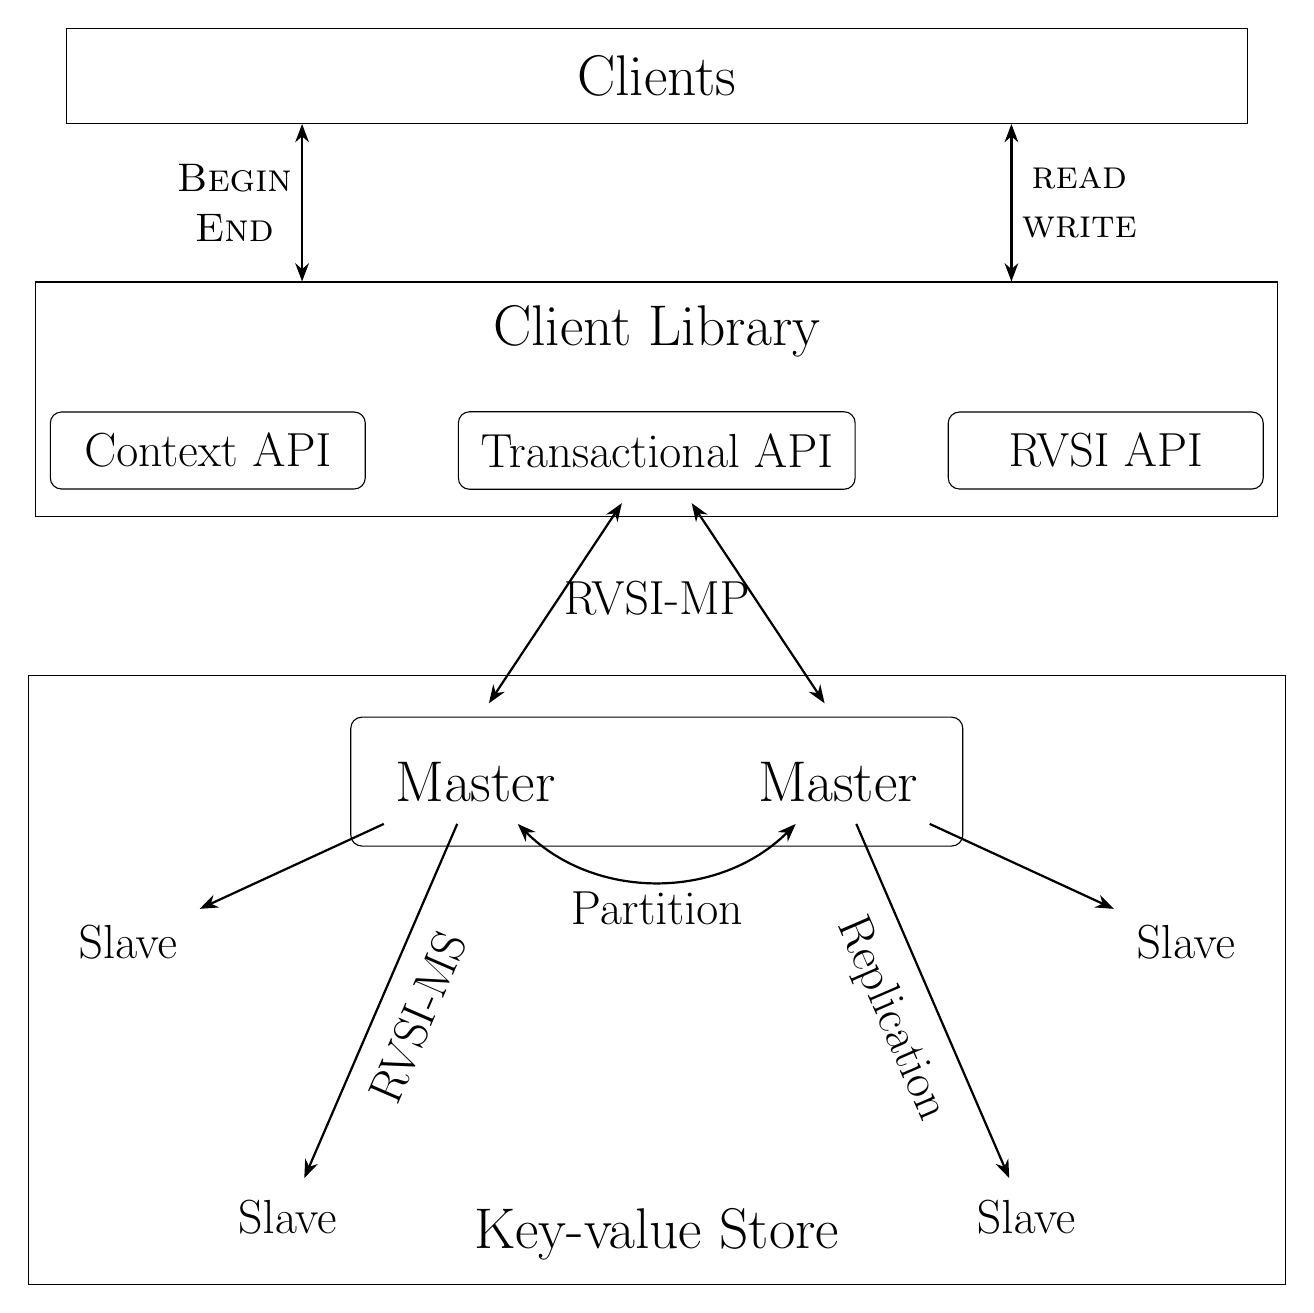
\begin{tikzpicture}[]
  
% client library: transactional api + rvsi api + context api
\begin{scope}[clib/.style = {draw, rectangle, rounded corners, font = \LARGE, inner sep = 8pt, minimum width = 4cm}]
  \node (tx-api) [clib, outer sep = 5pt] at (0,0) {Transactional API};
  \node (rvsi-api) [clib, right = of tx-api] {RVSI API};
  \node (ctx-api) [clib, left = of tx-api] {Context API};

  % client library text
  \node (client-library-text) [font = \huge, above = 0.40cm of tx-api] {Client Library};

  % surrounding
  \begin{pgfonlayer}{background}
    \node (client-library-surrounding) [rectangle, draw, inner sep = 5pt, fit = (tx-api) 
    (rvsi-api) (ctx-api) (client-library-text)] {};
  \end{pgfonlayer}
\end{scope}

% distributed transaction:
\begin{scope}[master/.style = {rectangle, rounded corners, font = \huge, inner sep = 8pt}, 
	dist-tx/.style = {>=Stealth, <->, outer sep = 3pt, thick}]
  % two masters
  \node (master-left) [master, below left = 3.0cm and 1.0cm of tx-api.south] {Master};
  \node (master-right) [master, below right = 3.0cm and 1.0cm of tx-api.south] {Master};
  \draw [>=Stealth, <->, bend right = 45, thick] (master-left) to node[font = \LARGE, sloped, below] {Partition} (master-right);

  % master surrounding
  \begin{pgfonlayer}{background}
    \node (master-surrounding) [rectangle, rounded corners, draw, inner sep = 8pt, outer sep = 5pt,
		fit = (master-left) (master-right)] {};
  \end{pgfonlayer}

  % distributed transaction
  \draw [dist-tx] (tx-api) to (master-surrounding.155);
  \draw [dist-tx] (tx-api) to (master-surrounding.25);
  \node (dist-tx-text) [font = \LARGE, above = 1.00cm of master-surrounding.north, align = center] {RVSI-MP};
\end{scope}

% replication
\begin{scope}[slave/.style = {rectangle, rounded corners, font = \LARGE, inner sep = 8pt}, 
  	rep/.style = {>=Stealth, ->, draw, thick}]
  % slaves of master-left
  \node (slave-left-above) [slave, below left = 1.0cm and 2.2cm of master-left] {Slave};
  \node (slave-left-below) [slave, below right = 2.5cm and 0.20cm of slave-left-above] {Slave};
  \draw [rep] (master-left) to (slave-left-above);
  \draw [rep] (master-left) to node[sloped, font = \LARGE, above] {} node[sloped, font = \LARGE, below = 5pt] {RVSI-MS} (slave-left-below);
  % slaves of master-right
  \node (slave-right-above) [slave, below right = 1.0cm and 2.2cm of master-right] {Slave};
  \node (slave-right-below) [slave, below left = 2.5cm and 0.20cm of slave-right-above] {Slave};
  \draw [rep] (master-right) to (slave-right-above);
  \draw [rep] (master-right) to node[sloped, font = \LARGE, above] {} node[sloped, font = \LARGE, below = 5pt] {Replication} (slave-right-below);
\end{scope}


% data store surrounding
\begin{pgfonlayer}{background}
  \node (datastore-surrounding) [draw, rectangle, inner sep = 10pt, 
	fit = (master-left) (master-right) (slave-left-above) (slave-left-below) (slave-right-above) 
	  (slave-right-below) (master-surrounding)] {};
\end{pgfonlayer}

% data store text
\node (datastore-text) [above = 0.20cm of datastore-surrounding.south, font = \huge] {Key-value Store};

% client
\begin{scope}[access/.style = {>=Stealth, <->, thick}]
  \node (client) [above = 2.0cm of client-library-surrounding, draw, font = \huge, rectangle, inner sep = 10pt, minimum width = 15.0cm] {Clients};
  \coordinate (client-left) at ($ (client.south west) ! 0.20 ! (client.south east)$);
  \coordinate (client-right) at ($ (client.south west) ! 0.80 ! (client.south east)$);
  \draw [access] (client-left) to node [left, font = \Large, align = center] 
	{\textsc{Begin}\\\textsc{End}} (client-left |- client-library-surrounding.north);
  \draw [access] (client-right) to node [right, font = \Large, align = center] 
	{\textsc{read}\\\textsc{write}}(client-right |- client-library-surrounding.north);
\end{scope}
\end{tikzpicture}
\end{document}